
\documentclass[a4paper,twoside,kulak]{kulakreport}

\renewcommand{\thesection}{\arabic{section}}

\usepackage[dutch]{babel}
\usepackage{hyperref}
\usepackage{graphicx}
\usepackage{flafter}
\usepackage{amsmath, amssymb, amsthm}
\usepackage{siunitx}
\usepackage{pdfpages}
\usepackage{subfiles}
\usepackage{wrapfig}
\usepackage{float}
\usepackage{url}
\usepackage{translator}
\usepackage{pdfpages}
\usepackage{siunitx}
\uselanguage{Dutch}
\usepackage{longtable}
\usepackage{booktabs}
\usepackage{enumitem}
\usepackage{array}
\providetranslation[to=Dutch]{Figure}{Figuur}

\usepackage{etoolbox}
\usepackage{booktabs}
\usepackage{xstring}
\usepackage{xcolor,colortbl}
\definecolor{gray1}{gray}{0.7}
\definecolor{gray2}{gray}{0.85}
\definecolor{gray3}{gray}{0.95}

% counting system		
\newcounter{counter}
\newcounter{subcounter}
\newcounter{subsubcounter}
\newcommand{\teller}{
	\stepcounter{counter}
	\setcounter{subcounter}{0}
	\setcounter{subsubcounter}{0}
	\thecounter}
\newcommand{\subteller}{
	\stepcounter{subcounter}
	\setcounter{subsubcounter}{0}
	\thecounter.\thesubcounter}
\newcommand{\subsubteller}{
	\stepcounter{subsubcounter}
	\thecounter.\thesubcounter.\thesubsubcounter}

% row	
\newcommand{\row}[3]{
	\IfEqCase{#1}{
		{1}{\teller & #2 & \IfEqCase{#3}{{0}{niet OK}{1}{OK}} \\}
		{2}{\subteller & #2 & \IfEqCase{#3}{{0}{niet OK}{1}{OK}} \\}
		{3}{\subsubteller & #2 & \IfEqCase{#3}{{0}{niet OK}{1}{OK}} \\}
	}[PackageError{row}{Undefined option to row: #1}]}





\faculty{Groep Wetenschappen \& Technologie}
\group{\texttt{X0B54a} -- Probleemoplossen en ontwerpen, deel 2}
\title{Ontwerpproces van een zelfrijdende wagen}
\subtitle{Eindverslag}
\author{Team 4: Team R2D2}
%\emailaddress{}
\institute{Matthijs Deforche, Karl Van Holder, Thomas Varheust, Kobe De Weerdt, Yaron Verhulst \\ Kevin Truyaert, Benjamin Maveau, Martijn Boussé}

\date{Academiejaar 2020 -- 2021}
\address{\textbf{\theauthor}\\
	Groep Wetenschap \& Technologie \\
	KU Leuven Kulak           \\
	Etienne Sabbelaan 53, 8500 Kortrijk
}

\begin{document}
	\titlepage
	
	
	
	\renewcommand*\contentsname{Inhoud}
	\tableofcontents
	

	\newpage
	
	\section{Inleiding}
	
	Het principe van zelfrijdende wagens is vandaag de dag geen item meer dat alleen in de toekomst mogelijk is. Er zijn al verschillende bedrijven volop aan de slag met de ontwikkeling van zelfrijdende wagens. Een ideaal voorbeeld hiervan is de autofabrikant Tesla. Vele ongevallen worden nog steeds veroorzaakt door de mens, dus lijken zelfrijdende wagens hiervoor een ideale oplossing. Om dit mogelijk te maken is het van essentieel belang om betrouwbare zelfrijdende wagens te ontwikkelen. Dit semesterproject laat ons toe om kennis te maken met de werking en principes van kleine robotwagentjes. 
	
	Het concept van $Smart$ $city$ ofwel slimme stad is een concept dat we in dit project zullen gebruiken.  $Smart$ $city$ is een stad waar alles bestuurd en beheerd wordt door informatietechnologie. Mobiliteit is een heel belangrijk deelaspect van het concept. Men wilt het verkeer zo efficiënt mogelijk in de stad regelen zodat er zo weinig mogelijk conflicten, ongevallen, filevorming enzovoort zijn.  Dit semester zullen we een zelfrijdend robotwagentje ontwerpen dat zelfstandig door een modelstad zal rijden. Het moet in staat zijn om verkeerslichten te kunnen interpreteren, juiste handelingen te kunnen uitvoeren zoals afslaan of rechtdoor rijden en het zal obstakels zoals voorliggers moeten kunnen ontwijken. Een vlotte verkeerssituatie in $Smart$ $city$ is cruciaal en dit is dan ook het doel van dit project. Onze auto zonder problemen en vlot laten rijden in de modelstad net zoals in het concept. 

	%%hoofdtekst
	
	\newpage
	
	
	\section{Klantenvereisten}

	De constructie van onze wagen moet aan een budget voldoen van 3500 eenheden. Er is een materiaallijst beschikbaar die we kunnen raadplegen om onderdelen te bestellen. \\

	Onze auto moet een geïmplementeerd traject kunnen volgen via een lijn die op de ondergrond is aangebracht. Deze verschilt qua intensiteit met de ondergrond zodat de auto de lijn kan herkennen. Het traject bevat ook meerdere kruispunten met verkeerslichten. Onze auto moet deze kunnen interpreteren en gepast reageren op het rode of groene licht. Om te kunnen stoppen bij het rode licht zal onze auto een dikke stoplijn moeten kunnen detecteren. \\

	Om het traject te volgen zal onze auto dus moeten kunnen rijden en draaien. Ook stoppen is belangrijk. Onze auto moet namelijk voorliggers kunnen detecteren en op tijd stoppen om een botsing te vermijden. Er wordt verwacht dat het volledige traject foutloos uitgereden kan worden op een aanvaardbaar tempo. \\

	Voor onze auto het traject op kan, zullen we ook een noodstop moeten uitvoeren. Dit zal via commando's van een computer moeten gebeuren.

	\newpage
	\section{Ontwerpspecificaties}
	 	De verkeerslichten kunnen interpreteren: stoppen bij een rood licht, doorrijden bij een groen licht.\\
	 De hoogte van het verkeerslicht gemeten vanaf de grond tot aan het middelpunt van het verkeerslicht is 75~mm. Het verkeerslicht heeft een knipperfrequentie van 1~Hz. Een technische tekening van het kruispunt is te zien op Figuur \ref{fig: verkeerslicht}.
	 \bigskip
	 
	 
	 
	 Een geïmplementeerd traject kunnen volgen / stoplijn detecteren.\\
	 De ondergrond van het traject zal ofwel donker ofwel helder zijn. De kleur van de lijnen die de auto moet volgen zal afhangen van wat de kleur van de ondergrond is. Het zal het omgekeerde zijn waardoor het verschil duidelijk is. Er zijn ook nog verschillen in de soorten lijnen die op de ondergrond aangebracht zullen worden. De breedte van een volglijn is 25~mm en de breedte van een stoplijn is 50~mm. De kruispunten liggen op 1000~mm van elkaar en het bovenaanzicht van een kruispunt is te zien op Figuur \ref{fig: kruispunt}. 
	 
	 
	 \bigskip
	 
	 
	 Commando's van een computer kunnen volgen.\\
	 Vooraleer onze auto het traject mag oprijden, moeten we eerst op afstand een noodstop kunnen uitvoeren. 
	 
	 
	 
	 \bigskip
	 
	 De auto moet aan een bepaald budget voldoen.\\
	 Er is een budget van $3500$ eenheden beschikbaar. Dit budget kunnen we gebruiken om materiaal aan te kopen op de site: http://www.irkulak.be/po2/.
	 Verder kunnen we het budget ook nog gebruiken om onze eigen ontwerpen te 3D-printen. 
	 
	 \bigskip
	 Het volledige traject foutloos kunnen afleggen met een aanvaardbaar tempo.\\
	 De wagen heeft een maximumbreedte van 250~mm, een maximumhoogte van 300~mm en een minimumhoogte van 75~mm.
	 
	 \newpage
	
	\section{Teamverantwoordelijkheden}
		\begin{tabular}{|c||l|l|l|l|}
		\hline
		Naam & Deforche Matthijs & De Weerdt Kobe & Van Holder Karl   \\ \hline \hline
		
		Penningmeester             &  &x &   \\ \hline
		Teamleider                 &  &  &x   \\ \hline      
		Notulist                   &  &  &    \\ \hline
		3D-modelleren              &  &  &   \\ \hline
		Programmeren               &x &  &x   \\ \hline
		Verantwoordelijke bouwen   &  &  &x  \\ \hline
		Verantwoordelijke aankopen &  &x &   \\ \hline
		Presentatie                &x &x &    \\ \hline
		
		
	\end{tabular}
	
	\bigskip
	
	\begin{tabular}{|c||l|l|}
			\hline
		Naam & Thomas Varheust & Yaron Verhulst   \\ \hline \hline
		
		Penningmeester             &  &    \\ \hline
		Teamleider                 &  &     \\ \hline      
		Notulist                   &x  &      \\ \hline
		3D-modelleren              &x  &x     \\ \hline
		Programmeren               & &     \\ \hline
		Verantwoordelijke bouwen   &x  &    \\ \hline
		Verantwoordelijke aankopen &  &   \\ \hline
		Presentatie                & &x    \\ \hline
	\end{tabular}
	
	 
\newpage
	
	\section{Ontwerp}
	\subsection{Onderdelen}
	We hebben keuze tussen een Raspberry Pi en een NI MyRio als microcontroller voor de auto en kiezen voor de NI MyRio. Voornamelijk het porgrammeren heeft ons overtuigd om met de MyRio controller te werken. 
	We kunnen op deze manier namelijk voor het volledige programmeerwerk LabVIEW gebruiken wat zorgt voor een naadloze integratie aangezien we sowieso LabVIEW gebruiken op de demo als $interface$. Het lijkt ons een voordeel als we zowel het programmeren in LabVIEW als de demo kunnen uitvoeren in dezelfde programmeertaal. 
	Daarnaast laat de MyRio ook analoge sensoren toe. 
	Eén van die sensoren is de afstandssensor die een bereik heeft van 80~cm, tegenover de 10~cm van de digitale variant die we ter beschikking hebben. Wanneer het wagentje een voorligger detecteert op een grotere afstand, kunnen we beter onze snelheid aanpassen aangezien er meer 'tijd' is om te reageren. Als er door een fout in het programmeerwerk het algoritme veel tijd vraagt om te kunnen stoppen, is het een voordeel als we een afstandssensor gebruiken die voorliggers op een grotere afstand detecteert. 
	We gebruiken voor de andere sensoren ook de analoge versies zodat we tijdens het programmeren enkel rekening hoeven te houden met dezelfde verwerking van de sensoren. 
	Aangezien de NI MyRio een power input nodig heeft van 6-16 Volt, kan de powerbank (met een output van 5~V) niet gebruikt worden.  Door TWEE Lithium-ion batterijen van 3,6 Volt te kiezen en deze in serie te schakelen is het wel mogelijk om een geschikte spanning voor de power-input te verkrijgen.
	\bigskip
	Als persoonlijke touch kozen we om geen $MakerBeams$ te gebruiken.
	In plaats daarvan hebben we dus een chassis nodig en het beste voor ons is het `rechthoekig zwart chassis' omdat we graag voldoende plaats hadden voor alle componenten te bevestigen. Het rechthoekig chassis heeft namelijk een oppervlakte van \SI{137.6}{\milli\metre\squared} , het rond heeft een oppervlakte van ongeveer \SI{126.7}{\milli\metre\squared}. 
	Ook kunnen we de wagen stabieler maken door het zwaartepunt te verlagen wanneer we de onderdelen meer kunnen uitspreiden. 
	Er is ook een `universeel chassis' dat we kunnen gebruiken, maar aangezien het 50 eenheden meer kost, hebben we beslist om deze niet te gebruiken. 
	\bigskip
	Voor wielen en motoren gaan we voor een $ball caster$. Als we enkel de balcaster gebruiken, zal ons chissis niet horizontaal liggen aangezien de balcaster minder hoog is dan de wielen. Daarom hebben we de extra componenten gebruikt bij de $ball caster$ die voor een verhoging zorgen. Hierdoor ligt ons chassis wel horizontaal. 
	Deze twee wielen drijven we aan met twee van de `Micro Metal Gear Motor 50:1 HP'.
	Deze heeft een drie millimeter as, wat compatibel is met onze gekozen wielen en heeft een gemiddeld vermogen, voldoende om de wagen te doen stoppen en opnieuw te versnellen.
	Omdat deze motoren niet meer beschikbaar waren wanneer wij onze bestelling konden plaatsen kozen we voor de `Micro Metal Gear Motor 100:1 HP', deze is redelijk gelijkaardig, maar heeft een ander vermogen. 
	Samen met deze motoren kozen we twee motorbeugels om de motoren aan het chassis te kunnen bevestigen en de `Dual Drive DRV8833' zodat we beide motoren tegelijk kunnen aansturen.
	Vooraleer we alles definitief solderen, willen we eerst het wagentje kunnen testen met de sensoren. Daarom kozen we voor een klein $breadboard$ zodat we de sensoren aan de microcontroller kunnen conecteren zonder dat we ze definitief verbinden door het solderen. De kleine versie was groot genoeg voor alle sensoren te kunnen verbinden, daarom kozen we voor het kleine aangezien het minder eenheden kost van ons budget. 
	\newpage
	\subsection{Assemblage}
	\begin{figure}[h]
		\centering
		\includegraphics[width=1.2\textwidth]{KS®wagen1.3}
		\caption{CAD-ontwerp van de wagen, samengesteld uit \textit{.par-onderdelen}, gezien vanuit de rechterbovenhoek.}
		\label{fig: wagen}
	\end{figure}
	
	\begin{figure}[h]
		\centering
		\includegraphics[width=1.2\textwidth]{KS®skelet.4}
		\caption{Het 3D-geprinte onderdeel \textit{Skelet van de wagen} }.
		\label{fig: skelet}
	\end{figure}
\newpage
	Het 3D-model van de wagen is te zien in Figuur \ref{fig: wagen}.
	De MyRio-microcontroller zit in een soort doos. Deze is relatief groot en wanneer we deze op het chassis zouden bevestigen, gingen sommige poorten achter de wielen zitten en zouden we deze dus niet kunnen gebruiken. Daarom hebben we ervoor gekozen om de MyRio hoger te plaatsen zodat alle poorten vrij zijn. In Figuur \ref{fig: skelet} is het 3D-model te zien dat we ontworpen hebben dat op het chassis bevestigd kan worden. Dit ontwerp laat ons ook toe om de MyRio hoger dan de wielen te plaatsen zodat we alle poorten kunnen gebruiken. Dit model is ook voorzien van een plaats waar we de kleurensensor aan kunnen bevestigen. Deze hangt op een hoogte dat overeenstemt met de hoogte van de verkeerslichten. Namelijk een hoogte van 75~mm. Verder bevindt de kleurensensor zich op een horizontale afstand van 25~mm ten opzichte van het verkeerslicht en op 65~mm van de symmetrieas van het chassis. Ook aan de voorkant van ons 3D-model hebben we een plaats voorzien waar we de afstandssensor aan kunnen bevestigen. 
 	Omdat de MyRIO relatief zwaar is ten opzichte van de andere onderdelen, zorgt deze keuze ervoor dat het zwaartepunt van de wagen hoger komt te liggen. Om te voorkomen dat het zwaartepunt te hoog zou liggen, plaatsen we de batterijen centraal op het chassis onder de MyRio. De reflectiesensor wordt vooraan in het verlengde van het chassis bevestigd via de $reflectiesensorhouder$. Dit is een onderdeel dat we zelf ge-3D-print hebben omdat we ervoor gekozen hebben om geen $MakerBeams$ te gebruiken. In Figuur \ref{fig: wagen} is de houder vooraan aan de wagen bevestigd. Omdat de afstandssensor objecten waarneemt vanaf 80~mm hebben we besloten deze op 35~mm van de voorkant van het chassis te plaatsen. Hierdoor kan de auto op een gepaste afstand een tegenligger detecteren.  De sensoren maken verbinding met de MyRIO via de printplaat, deze is bovenaan op de MyRio bevestigd. Het elektrisch circuit is te zien in Bijlage \ref{sec: circ}. 
	
\section{Software}

\subsection{flowchart moet nog aangevuld worden}

we moeten eerst met behulp van flowchart/stroomdiagram het algemene idee uitleggen vd software
dit moet nog geschreven worden

\subsection{Lijnvolgalgoritme}
Het lijnvolgalgoritme werkt volgens een eenvoudig principe dat voorgesteld wordt in Figuur \ref{fig: lijnvolg}.
Het parcours bestaat uit donkere lijnen op een witte ondergrond. Bij het volgen van deze lijnen maken we gebruik van de `QTR-8A analoge reflectie sensor array'.
De aansluiting hiervan op de microcontroller kan je zien in Bijlage \ref{sec: circ}. De sensor heeft acht lichtgevoelige sensoren. We hebben ons lijnvolgalgoritme gebaseerd op het feit dat men aan de ene kant van de sensor meer zwart ziet dan aan de andere wanneer die niet evenwijdig met de lijn rijdt. Wanneer men meer zwart ziet aan de linkerkant van de sensor, moet men naar links draaien (dit door de linkermotor trager te doen draaien). Wanneer men echter meer zwart ziet aan de rechterkant van de sensor, moet men naar rechts draaien (dit door de rechtermotor trager te doen draaien ). Als men aan beide zijden even veel zwart detecteert, moet men rechtdoor blijven rijden. Dit algoritme komt tot een einde wanneer beide kanten even veel zwart ervaren en deze waardes tezamen veel groter zijn. Dit betekent dat er een stopstreep is, en men dus moet stoppen. 

\begin{figure}
	\centering
	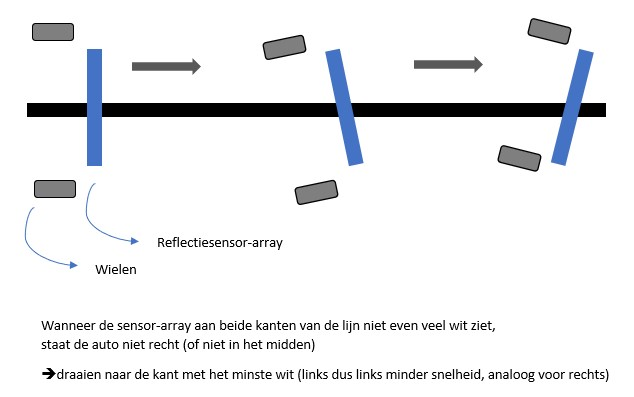
\includegraphics[width=.84\textwidth]{pref2}
	\caption{Het lijnvolgalgoritme laat ons robotwagentje toe om zijn traject te corrigeren indien nodig. Wanneer er links meer wit te zien is, zal het algoritme de wagen naar rechts laten draaien zodat hij de lijn correct volgt. Dit door de linkse motor sneller te laten  }
	\label{fig: lijnvolg}
	
\end{figure}
\subsection{Licht herkennen}
Dit algoritme treedt pas in werking als het wagentje een stopstreep detecteert. Dit is zo wanneer de zes sensoren van de reflectiesensor zwart detecteren (zoals in
vorige paragraaf beschreven). 
We kozen ervoor om met de kleurensensor de roodwaardes te meten, omdat we proefondervindelijk hiervoor betere waardes kregen. We kijken of het licht rood knippert met behulp van statistiek. We krijgen ongeveer 10 waardes per seconde en bundelen telkens 50 opeenvolgende waardes, hierop berekenen we de standaardafwijking. Wanneer het rode licht niet brand, meten we theoretisch gezien allemaal dezelfde waarden en is de standaardafwijking gelijk aan nul. Wanneer het rode licht knippert krijgen we in onze steekproef hoge en lage waardes, hierdoor is de standaardafwijking groter. Wanneer we een standaardafwijking hebben die lager is dan een proefondervindelijk bepaalde waarde gaan we ervan uit dat het licht niet rood knippert en de wagen door kan rijden. Zolang de standaardafwijking niet lager is dan deze bepaalde waarde blijft de wagen wachten.

\subsection{Andere wagen herkennen en versnellen/vertragen}

Met de afstandssensor kunnen we de afstand tot een voorliggende wagen detecteren. Wanneer de afstand te klein is, gaat de wagen vertragen. Als echter bij het vertragen de kritieke minimale snelheid overschreden wordt (dus nog minder dan de minimale), dan stopt onze wagen (dit is wanneer een andere wagen voor ons stilstaat). Wanneer de snelheid boven een bepaalde waarde is, neemt hij de 'ideale snelheid' aan.

\subsection{Draaien op kruispunt}
We maken een ondersheid tussen drie gevallen; linksaf, rechtsaf en rechtdoor. Bij linksaf moeten we eerst 375mm rechtdoor rijden, dan 90graden naar links draaien om de as van de wagen en tenslotte meer dan 375 mm rechtdoorrijden om dan weer de lijn te volgen.

Bij rechtsaf moet men eerst 125mm rechtdoorrijden, dan 90graden naar rechts draaien om de as van de wagen en tenslotte meer dan 125mm rechtdoorrijden om dan weer de lijn te volgen. Bij rechtdoor moet men meer dan 500mm rechtdoorrijden om dan vervolgens de lijn te volgen. bij deze drie gevallen moet men tijdens het uitvoeren ervan rekening houden of er al dan niet een voorligger zich binnen de zeer kritische gevarenzone bevindt (dit wil zeggen dat de ander wagen voor de een of andere reden stilstaan op het kruispunt)

\subsection{Handmatige Besturing}
Om de controle manueel over te nemen sturen we de motoren rechtstreeks aan. Dit stellen we voor met behulp van twee sliders in LabVIEW. Later zullen we aan die sliders concreet een invulling voor geven om op de test te gebruiken.

\subsection{Implementatie traject}

Vanaf het moment dat we ons traject kennen, kunnen we aan de hand van de vorige algoritmes ons parcours samenstellen. De flowchart van ons programma is terug te vinden in bijlage \ref{sec: flowchart}.

\subsection{Concrete implementatie}
\bigskip
Het hele LabVIEW-programma, gebruikmakend van de voorgenoemde functies splitsen we op in twee stappen:

De eerste stap is wat de auto moet doen tijdens het rijden. Hier moet de auto tegelijk de lijn op de grond volgen, 
een goede afstand tot zijn voorligger behouden (wat dus inhoudt dat die de voorligger moet detecteren en aan de hand van de afstand tot die voorligger zijn snelheid moet aanpassen) 
en de auto moet ook nog eens comfortabel kunnen stoppen,en dus niet te snel rijden, wanneer die een stopstreep detecteert. 
De input voor de snelheid komt van de motoren, de input voor de afstand tot de voorligger komt van de afstandssensor, de lijn en stopstreep detecteren we met de reflectiesensorarray en tot slot het verkeerslicht (dat besproken zal worden in de volgende stap) detecteren we met de kelurensensor.

De tweede stap begint bij de stopstreep van bij het eindd van stap één. 
Wanneer de auto gestopt is aan de stopstreep moet die een verkeerslicht detecteren en daar gepast opreageren, nadat het groen licht geworden is moet die dus over het kruispuntdraaien. 
Daarna moet die een bocht nemen of rechtdoor rijden aan de hand van een vooraf opgesteld parcours. 
Na deze stappen is het algoritme klaar en begint hij weer met stap één.
	
	\subsection{Implementatie traject}
	
	Vanaf het moment dat we ons traject kennen, kunnen we aan de hand van de vorige algoritmes ons parcours samenstellen. De flowchart van ons programma is terug te vinden in bijlage \ref{sec: flowchart}.
	


\section{Resultaten}
\subsection{Financieel raport}

Het gespendeerd budget is terug te vinden in Bijlage \ref{sec: finrap}.
Het grootste deel van het budget ging naar de aankoop van onderdelen voor onze wagen. Deze onderdelen zijn van essentieel belang aangezien we zonder deze onderdelen de opdracht niet goed kunnen uitvoeren. Het budget dat we hieraan gespendeerd hebben, was een verantwoorde beslissing. Voor het testen van de wagen hebben we een breadboard gekocht. Dit was voor ons een noodzakelijke aankoop aangezien we verschillende sensoren kunnen testen zonder dat we eerst alles definitief moeten solderen. 
Ten slotte is een groot deel van het budget gespendeerd aan de positie om aankopen te mogen doen. Het was voor ons belangrijk een hoge positie te krijgen zodat we meer keuzemogelijkheden hadden bij de aankoop van onderdelen. Aangezien er vijf MyRio- en vijf Raspberry Pi-microcontrollers waren, wisten we niet met zekerheid of we een MyRio-microcontroller konden krijgen. Daarom hebben we voor elke soort microcontroller een overzicht gemaakt met de onderdelen die we ernaast nog wilden aanschaffen. Op basis hiervan hadden we een idee van welk budget er nog over was voor de bieding en de 3D-prints. Zo konden we een gepast budget uittrekken voor de bieding rekening houdend met onverwachte aankopen en 3D-prints. 

\subsection{Ontwerp}
Tijdens het testen en tijdens de demo bleek dat ons ontwerp goed gewerkt heeft. De afstandssensor heeft goed de voorliggers kunnen detecteren dus het was op de correcte plaats geplaatst op ons 3D-model. De auto kon goed de lijnen volgen, dus onze $reflectiesensorhouder$ is opnieuw correct geplaatst en ontving geen hinder van andere onderdelen van het wagentje. Tijdens het testen, reed de auto plots snel vooruit en viel zo van tafel. Hierdoor is het onderdeel waar de kleurensensor aan vastging, afgebroken. Dit hebben we proberen te lijmen en vast te hangen met plakband. Wanneer deze hersteld was, was de houder van de kleurensensor een geslaagd onderdeel aangezien de kleurensensor de verkeerslichten kon interpreteren. Tijdens het testen en de demo merkten we dat de bocht naar rechts tamelijk scherp was en dat er onderdelen zoals de draden van de auto bleven haperen aan het kruispunt. Mocht er eventueel meer tijd geweest zijn, konden we dit aanpassen in ons ontwerp waardoor er geen haperingen waren bij de bocht naar rechts. De wagen heeft tijdens de demo geen elektrische problemen gehad, dus het soldeerwerk heeft goed gefunctioneerd. Door alle draden en de printplaat leek ons wagentje bovenaan wat rommelig. Indien er meer tijd ter beschikking was, zouden we nog een oplossing hiervoor gevonden willen hebben. 

\subsection{Software}
Tijdens de demo en het testen bleek dat de auto goed de lijnen kon volgen. Het lijnvolgalgoritme was een goede implementatie en we hebben hier weinig problemen bij ondervonden. De auto kon goed tegenliggers registreren en stoppen indien nodig, dus ook het programma om tegenliggers te registreren was een goede implementatie. Bochten nemen lukte niet helemaal perfect. Sommige kruispunten werden goed genomen, maar de andere lukten niet altijd. Onze auto draaide te scherp en reed soms tegen de constructie van de kruispunten.


\newpage
	\section{Bijlagen}
	
	\begin{figure}[h]
		\centering
		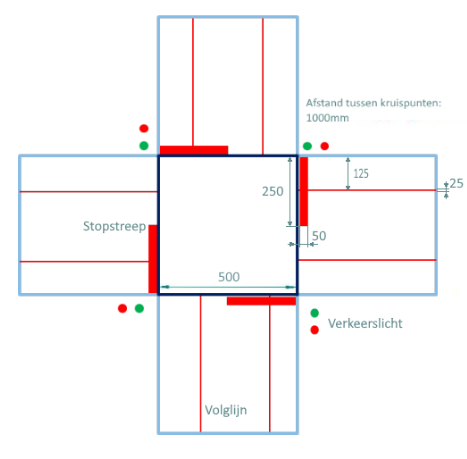
\includegraphics[width=.8\textwidth]{bovenaanzichtkruispunt}
		\caption{Bovenaanzicht kruispunt met relevante maten en items, aangepast vanuit \cite{Smart}.
		}
		\label{fig: kruispunt}
		
	\end{figure}
\newpage
	\begin{figure}[h]
		\centering
		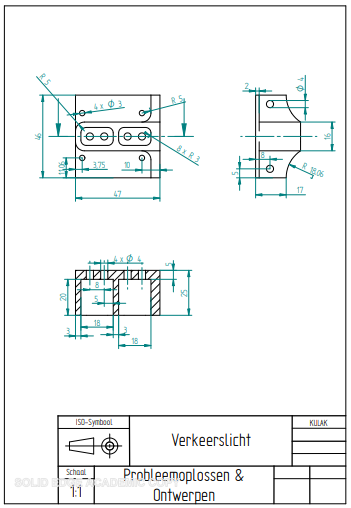
\includegraphics[width=.8\textwidth]{verkeerslicht}
		\caption{Technische tekening verkeerslicht, opgehaald van \cite{artikel1}. }
		\label{fig: verkeerslicht}
	\end{figure}
	
	

	\newpage

	

	\subsection{Takenstructuur}
	\label{sec: taken}
	
			
		\begin{table}
			\centering
			%\caption{Takenstructuur}
			
			Tabel 1: Takenstructuur
			
			% \vspace{\baselineskip}
			\begin{tabular}{p{1cm}p{12cm}c}
				
				
				\toprule
				Code & Taak & Status \\ 
				
				\midrule
				\row{1}{Inwerken}{1}
				\row{2}{Documenten op Toledo lezen}{1}
				
				\row{2}{Ontwerpen en plannen}{1}
				\row{3}{Materiaallijst maken}{1}
				\row{3}{Teamkalender maken}{1}
				\row{3}{Klantenvereisten opstellen}{1}
				\row{3}{Overzicht ontwerpspecificaties}{1}
				\row{3}{Takenstructuur}{1}
				\row{3}{Gantt-grafiek}{1}
				
				\midrule
				\row{1}{Ontwerpen met behulp van de computer}{0}
				\row{2}{3D modellen	(Solid parts)}{1}
				\row{3}{Wiel}{1}
				\row{3}{Motor}{1}
				\row{3}{Motorbeugel}{1}
				\row{3}{Chassis}{1}
				\row{3}{Ballcaster}{1}
				\row{3}{Printplaat}{1}
				\row{3}{Kleursensor}{1}
				\row{3}{Afstandssensor}{1}
				\row{2}{Assemblage (Assembly)}{1}
				
				
				\row{2}{Technische tekeningen (Drawing)}{0}
				
				\row{2}{Stuklijst}{0}
				
				\midrule
				\row{1}{Software}{0}
				\row{2}{Sturen/snelheid regelen}{1}
				\row{2}{Lijnvolgalgoritme}{1}
				\row{2}{Verkeerslichtinterpretatie}{1}
				\row{2}{Voorliggerdetectie}{1}
				\row{2}{Stoppen}{1}
				\row{2}{Vertragen}{1}
				\row{2}{Handmatig besturen}{1}
				\row{2}{Inputs vormgeven}{0}
				\row{2}{Outputs vormgeven}{0}
				\row{2}{Testen}{0}
				
				
				\midrule		
				\row{1}{Rapportering}{0}
				\row{2}{Tussentijds verslag}{1}		
				\row{3}{Nalezen}{1}
				\row{2}{Tussentijdse presentatie}{0}
				\row{3}{Structuur}{1}
				\row{3}{Presentatie maken}{0}
				\row{3}{Nalezen}{0}
				\row{3}{Inoefenen}{0}
				\row{2}{Eindverslag}{0}
				\row{3}{Structuur}{0}			
				\row{3}{Nalezen}{0}
				\row{2}{Eindpresentatie}{0}
				\row{3}{Structuur}{0}
				\row{3}{Presentatie maken}{0}
				\row{3}{Nalezen}{0}
				\row{3}{Inoefenen}{0}
				\bottomrule
			\end{tabular}
		
		\label{tab: taken}
		\end{table}
	\newpage
	
	
	\section{Gantt-grafiek \& Teamkalender}
	\label{sec: kale}
	\includepdf[pages = 7]{Team4_planning}
	\includepdf[pages = 8]{Team4_planning}
	\includepdf[pages = 9]{Team4_planning}
	\includepdf[pages = 10]{Team4_planning}
	\includepdf[pages = 11]{Team4_planning}
	\includepdf[pages = 12]{Team4_planning}
	\includepdf[pages = 13]{Team4_planning}
	
	
	
	\subsection{Visualisatie ontwerp}
	\label{sec: vis}
	

%%KS®wagen1.3

\subsection{Elektrisch circuit}
\label{sec: circ}

\subsection{Flowcharts}
\label{sec: flowchart}

\begin{figure}
	\centering
	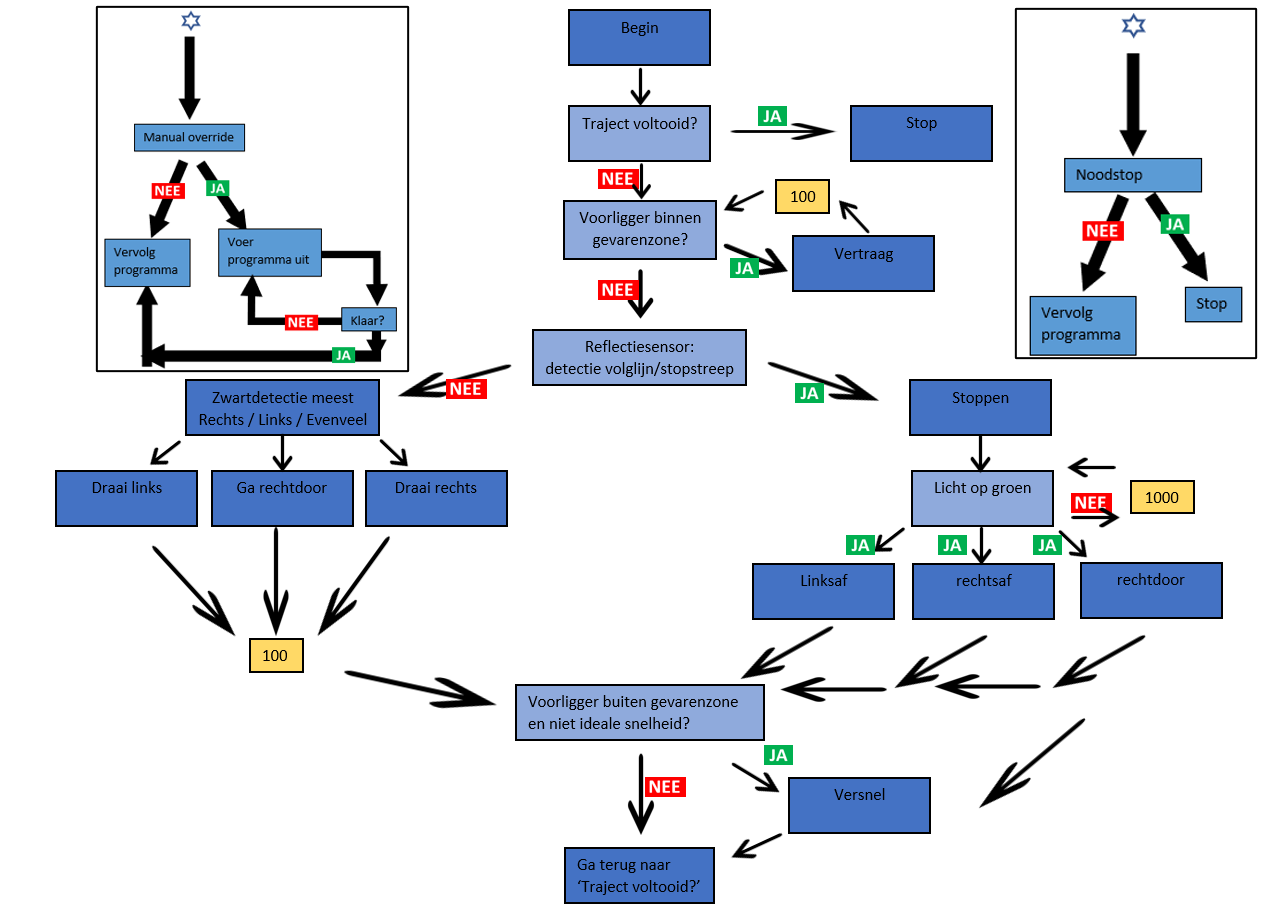
\includegraphics[width=1.3\textwidth]{fchart}
	\caption{De flowchart van ons algoritme. 
	}
	\label{fig: fchart}
	
\end{figure}

\newpage
	\subsection{Financieel Rapport}
	\label{sec: finrap}
	\subsection*{Hardware}
	
	\begin{table}[h]
		
	
	\begin{tabular}{l|r|r|r}
		Onderdeel& prijs per stuk & aantal & totale prijs \\
		\hline
		Micro Metal Gear Motor 100:1 HP&160 & 2 & 320 \\ 
		
		Dual Drive DRV8833 & 70 & 1 & 70 \\
		Optische afstandsensor (analoog) & 160 & 1 & 160 \\
		TCS34725 Kleur sensor BOB & 150 & 1 & 150 \\
		QTR-8A analoge reflectie sensor array & 150 & 1 & 150 \\
		Oplaadbare LITHIUM-ION & 90 & 2 & 180 \\
		NI MyRio  & 240 & 1 & 240 \\
		Breadboard Tiny & 40 & 1 & 40 \\
		Printplaat & 50 & 1 & 50 \\
		Totaal: 1360
	\end{tabular}
\caption{uitgaven hardware}
\label{tab: ess}
\end{table}
	
	
	\subsection*{Ontwerp}
\begin{table}[h]	
	\begin{tabular}{l|r|r|r}
		
		Onderdeel& prijs per stuk & aantal & totale prijs \\
		\hline
		Ball Caster &60 & 1 & 60 \\
		Wiel 60x8mm zwart &35 & 2 & 70 \\
		Robot Chassis Rechthoekig Zwart &70 & 1 & 70 \\
		
	\end{tabular}
	

	Totaal: 200
	
\caption{uitgaven ontwerp}
\label{tab: ontw}
\end{table}
	
	
	\subsection*{Assemblage}
\begin{table}[h]	
	\begin{tabular}{l|r|r|r}
		Onderdeel& prijs per stuk & aantal & totale prijs \\
		\hline
		Micro metal gear motor beugel &2 & 25 & 50 \\
		Skelet van de wagen &N.A & 1 & N.A\\
		Reflectie sensor houder &N.A & 1 & N.A\\
		
	\end{tabular}
	
	Totaal: 50
	
\caption{uitgaven assemblage}
\label{tab: ass}
\end{table}
	\subsection*{Onkosten}

\begin{table}[h]

	\begin{tabular}{l|r}
		kost& waarde \\
		\hline
		Bieding &1300 \\
		
		
	\end{tabular}
	\newline
	Totaal: 1300
\caption{uitgaven onkosten}
\label{tab: onk}
\end{table}
	
	\subsection*{Niet gebruikt}
	Totaal: 590
	
\begin{figure}[h]
	\centering
	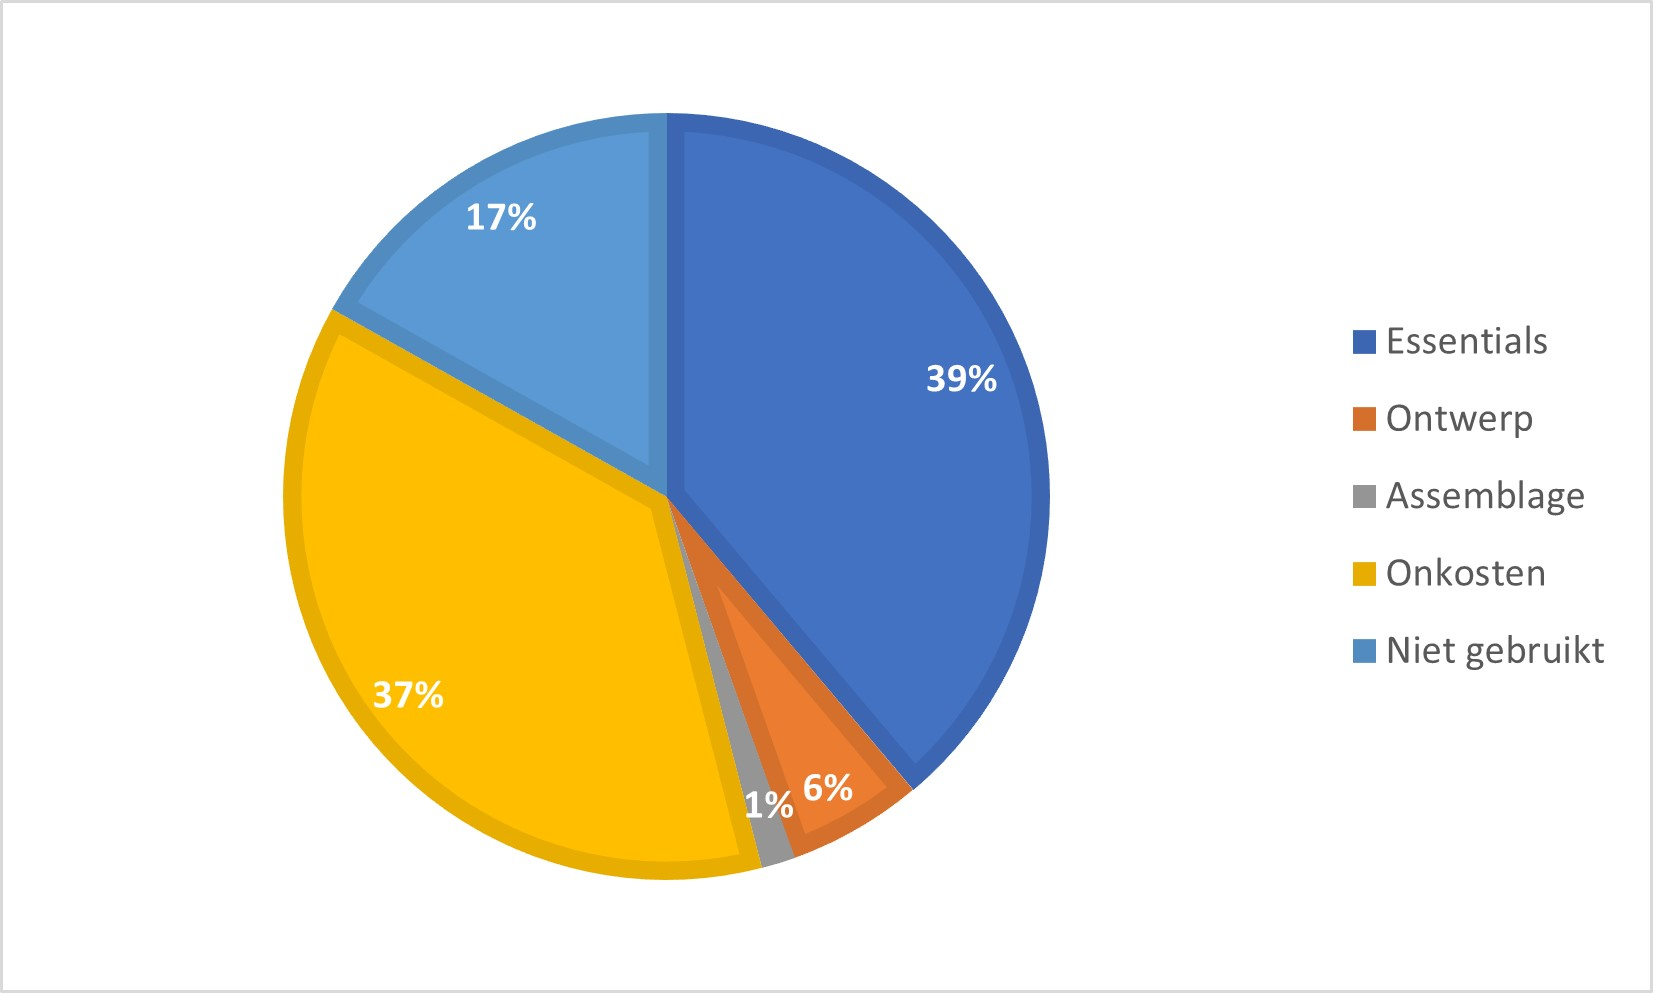
\includegraphics[width=1.2\textwidth]{pie}
	\caption{Visualisatie van de besteding van ons budget }
	\label{fig: pie}
\end{figure}
	
	
	
	
	
	
	
	%%referenties
	\bibliography{bibliografie_verslag.bib}
	\bibliographystyle{unsrt}
	
	
	
	%%Bijlagen
	
\end{document}